\documentclass[a4j]{jarticle}
\usepackage{graphicx}
\usepackage{ascmac}


\begin{document}

\title{計算機科学実験及演習2 \\ \bf ソフトウェア報告書1}
% ↓ここに自分の氏名を記入
\author{谷 勇輝 \\ \\入学年 平成27年 \\ 学籍番号 1029-27-2870}
\西暦
\date{提出日: \today} % コンパイル時の日付が自動で挿入される
\maketitle

\section{課題1}
\begin{screen}
 ステージパラメータおよび既存エージェントを様々に変更し動作を見る。また、エージェントプログラムの内容を理解する。以下の既に実装されているエージェン
トの1つを選び、ソースコードから動作を説明せよ。ソースコードは、ch . idsia . agents . controllers .[エージェント名]. java にある。\\
● ForwardAgent \\
● RandomAgent \\
● ScaredAgent \\
● ScaredShootyAgent 
\end{screen}
\subsection{実施内容}
\begin{description}
\item[(1)]~\\
 ステージパラメータ(seed、難易度、敵の有無、その他地形等の変数)と既存エージェントを様々に変更し、動作を観察した。
\item[(2)]~\\
 ch.idsia.agents.controllersパッケージ内に用意されたAgentプログラムのうち、
ForwardAgentについてソースコードと動作の比較からその内容を理解した。
\item[(3)]~\\
 各Agentプログラムに頻繁に登場する isMarioAbleToJump と isMarioOnGround の2つのパラメータについて理解を深めるため、以下のソースコードをAgentプログラムの適切な箇所にアサーションし、その内容について考察した。
\begin{verbatim}
System.out.println(isMarioAbleToJump + "/" + isMarioOnGround + 
                                 " = " + action[Mario.KEY_JUMP]);
\end{verbatim}
\end{description}
%%%
\subsection{実行結果}
\begin{description}
\item[(1)]~\\
 それぞれのパラメータについて、難易度、シードの値を様々に変更し観察し意味を理解した。
また、概ね自分の望むタイプのコースを用意できるようになった。
特記すべきパラメータについては以下に詳細を記述する。
	\begin{description}
	\item[Hill(丘)] ~\\
	デフォルトで全ての難易度で出現する。\\
	下からのジャンプを透過し、床として使用できる。\\
	marioAIOptions.setHillStraightCountメソッドでfalseに設定することで出現しなくなる。
	\item[Tubes(土管)] ~\\
	デフォルトで全ての難易度で出現する。 パックンフラワーの出現率は難易度で異なるように思われる。\\
	marioAIOptions.setTubesCountメソッドでfalseに設定することで出現しなくなる。
	\item [Gaps(落とし穴)] ~\\
	難易度1以上で出現する。\\
	marioAIOptions.setGapsCountメソッドをfalseにすることで出現しなくなる。\\
	難易度0では値をtrueにしても出現しない。
	\item [Cannons(砲台)] ~\\
	難易度2以上で出現する。\\
	marioAIOptions.setCannonsCountメソッドをfalseにすることで出現しなくなる。\\
	難易度1以下では値をtrueにしても出現しない。
	\item [DeadEnds(行き止まり)] ~\\
	デフォルトでは出現しない。\\
	難易度に関わらず、marioAIOptions.setDeadEndsCountメソッドで有無を操作できる。\\
	以下のいずれか、もしくは複数の地形が発生する。\\
	\\
	 ・マリオがジャンプによって越えることのできない、地面からの壁\\
	 ・上方画面外から続く、空中をふさぐ壁。\\
	 ・上記の2つの地形に、その壁に密着するように延びる地面を追加した鍵型の地形。\\
	\\
	袋路を形成する可能性があり、後戻りが必要になりうる。
	\end{description}
\item[(2)]
 \begin{description}
  \item[resetメソッド]~\\
   以下の五つの設定を行っている。
   \begin{enumerate}
   \item 配列actionの生成(中身はfalseで初期化されている)
   \item 要素RIGHTをtrueにする ~\\
     このAgentでは右ボタンは常に押された状態である。
  \item 要素SPEEDをtrueにする ~\\
     このAgentではダッシュ&ファイアは常に押された状態である。
  \item trueJumpCounterを0に初期化する
   \item trueSpeedCounterを0に初期化する~\\
     これらの2変数の内容については後述する。
   \end{enumerate}
  \item[getActionメソッド]~\\
    マリオの毎ターンの行動を定めている。まず、マリオが「危険状態」かどうかを判断する。DangerOfAnyメソッドがtrueで、進行方向1マス目がコインではないとき、それを「危険状態」としている。
    \begin{description}
    \item[危険状態の時]~\\
      マリオがジャンプ可能(isMarioAbleToJump==true)の時には要素JUMPをtrueとする。また、マリオが空中にいて(!isMarioOnGround==true)直前もジャンプキーを押している際はジャンプキーを押しつづける。
    \item[危険状態にないとき]~\\
      マリオはジャンプボタンを離す。
   \end{description}
     また、マリオの目の前が障害物で着地しているのにジャンプボタンを離しそこねた場合の詰みを防ぐため、17ターン連続でジャンプボタンを押している際はボタンを離すようになっている。
 \item[DangerOfAnyメソッド]~\\
以下のいずれかに当てはまる時、trueを返す。
   \begin{description}
      \item マリオの1マス前に2マス以上の穴がある。(これには空中も含まれる。)
      \item マリオの1マスまたは2マス前に障害物がある。
      \item マリオの1マスまたは2マス前に敵がいる。
      \end{description}
  \end{description}
\item[(3)]~\\
 一部を抜粋する。
\begin{verbatim}
<FowardJumprinAgent>
 ....
false/false = true
false/false = true
false/false = true
false/true = false
true/true = true
false/false = true
false/false = true
...
\end{verbatim}

\begin{verbatim}
<FowardAgent>
...
false/false = false
false/true = false
true/true = false
true/true = true
false/false = false
false/false = false
false/false = false
false/false = false
false/false = false
false/false = false
false/false = false
true/false = true
false/false = true
false/false = true
false/false = true
...
\end{verbatim}

\end{description}

%%%
\subsection{結論と考察}
\begin{description}
\item[(1)]~\\
ステージパラメータについては、以下の三つのタイプのパラメータがあると分類することができる。
\begin{enumerate}
\item 難易度に関わらずデフォルトで出現するもの ~\\
コイン、ブロック、丘、土管
\item 特定難易度以上でしか出現しないもの~\\
落とし穴、砲台
\item 値をtrueに設定した場合のみ出現するもの~\\
行き止まり、Flat、隠しブロック (隠しブロックについては未検証)
\end{enumerate}

 難易度とそれによるステージの変化については、続く課題を行う際に随時確認していきたい。
詳しく調査を行うことができたので、適宜適切なステージを構築し、人工知能プログラムの検証等に役立てたいと思う。

また、今回の分析をふまえ、Mainクラス内を望むステージを作り易いよう改良した。
\begin{verbatim}
public final class Main
{
public static final int  SEED = 30,
		  	DIFFICULTY = 0;

public static void main(String[] args)
{
    final MarioAIOptions marioAIOptions = new MarioAIOptions(args);
 
    //ステージパラメータ
    marioAIOptions.setLevelRandSeed(SEED);
    marioAIOptions.setLevelDifficulty(DIFFICULTY);

//  marioAIOptions.setDeadEndsCount(true);		//dead_ends
//  marioAIOptions.setHiddenBlocksCount(true);	//hidden_blocks
//  marioAIOptions.setFlatLevel(true);			//flat
   
//  marioAIOptions.setCoinsCount(false);		//coins
//  marioAIOptions.setHillStraightCount(false);	//hill
//  marioAIOptions.setBlocksCount(false);		//blocks
//  marioAIOptions.setTubesCount(false);		//tubes
//  marioAIOptions.setGapsCount(false); 		//gaps
//  marioAIOptions.setCannonsCount(false);		//cannons
    
    //敵の有無  
//  marioAIOptions.setEnemies("off");	//キラーとパックンのみ
//  marioAIOptions.setEnemies("g"); 	//クリボー
//  marioAIOptions.setEnemies("ggk");
    
    // エージェントの追加
    final Agent agent = new ForwardJumpingAgent();
    marioAIOptions.setAgent(agent);
    
    final BasicTask basicTask = new BasicTask(marioAIOptions);
    basicTask.setOptionsAndReset(marioAIOptions);
    basicTask.doEpisodes(1,true,1);
    System.exit(0);
}
}
\end{verbatim}

SEED,DIFFICULTYの値を変更しやすい位置に移し、各ステージパラメタをコメント扱いで待機させている。
例えば土管を消したいのであれば //tubes の位置のコメントを外せばすぐに実現できる。
\item[(2)]~\\
 ForwardAgentプログラムは、基本的な危機回避動作を組み込んだプログラムと言える。具体的には以下の三つに対応する事を目的としているようである。それぞれの観点から、実装のよい点と悪いところを述べる。
 \begin{enumerate}
  \item 障害物を回避し、ゴールまで到達すること。~\\
 ジャンプによっておおむね全ての障害物を回避できる。変数trueJumpCounterを利用した詰み防止も良く機能している。マリオがLARGEの状態の際に、高さの幅がブロックによって2に縮まった道が出現すると、小さなジャンプではなく大きなジャンプを選択してしまうことから詰みがおきてしまう。また、袋地に対しては完全に無力である。
 \item 敵を回避し、死亡しないこと。~\\
 単純に歩いてくる敵に対してはおおむね対処できる。着地位置に敵がいるかどうかの判定はしていないので、着地後に敵にぶつかることはままある。また、特に上から降りてくる敵に対して脆弱であり、大抵の死亡要因はこれである。
 \item 穴を回避し、死亡しないこと。~\\
 基本的な穴は回避できる。着地判定をしていないことから、大きなジャンプの先に穴が存在し死亡してしまうことは良く起きる。
  \end{enumerate}
 
レベル0のコースをクリアするだけの力はあるが、よりレベルの高いコースに対しては精度の高い実装が必要となる。また、コーディングも全体として甘く、目的にあったプログラムが書けているとは言い難い。getActionメソッド内の「~~=!1」の明らかなミスに加え(コインを危険として判断しないことを意図するならば~~!2が正しい)、ジャンプの最中も「穴」の危険があると判定してしまっている所など、精密さに欠けているところなどが改善すべき点と言える。
\item[(3)]~\\
 ForwardJumpingAgentは、できる限り大きなジャンプを行うエージェントである。着地の直後にジャンプボタンを離し、再びジャンプボタンを押す。

 アサーションしたログを確認すると、ジャンプ不可/着地済みの場合のみ要素JUMPがfalseになっているのが良く分かる。またマリオの状態は、基本的には以下の3ステップを繰り返すことが分かった。
\begin{enumerate}
 \item ジャンプ不可/空中
 \item ジャンプ不可/地上
 \item ジャンプ可能/地上
\end{enumerate}
 敵を踏む際も状態はジャンプ不可/空中である。また、ForwardAgentが観測した「ジャンプ可能/空中」となりうるのは確認できた限り以下の2つの場合に限られる。
\begin{enumerate}
 \item 壁づたいにいて、壁方向にキーを入れている時
 \item ブロックなどの先端を擦るように動いた時
\end{enumerate}
 前者はいわゆる「壁キック」可能な状態であり、この時にジャンプキーを入れると逆方向に飛び上がることができる。後者は既にブロックに乗っているか微妙な状態での判定のすれ違いによるものと考えられる。
\end{description}

%%\newpage

\section{課題2}
\begin{screen}
  上記のアルゴリズムを拡張し(穴をジャンプでよける、ブロックで進行が止められる状況を回避し)、
与えられた敵のないシーン(ch . idsia . scenarios . MainTask2 . java )でステージをクリアするエージェントを
実装し、クリアできることを確認せよ。どのようなプログラミングを行ったかのアイデアと実装方法をレポートで示すこと。
\end{screen}
\subsection{実施内容}
無駄な動きの少ない、美しく滑らかな動きを目指してマリオエージェントのプログラミングを行った。
 以下に重視した点を示す。
 \begin{description}
 
  \item[(1)クラス構造]~\\
 今後のエージェントの拡張、コードの複雑化を踏まえクラス構造を設計した。AIはコンピュータで人間の知能を模倣する技術であるという点を踏まえ、
  	モデルとして感覚神経・脳・運動神経(体)という人間の処理構造を使用し、それぞれOwnAgentSensesクラス、OwnAgentBrain抽象クラス、OwnAgentクラスとして実装している。
  	脳のクラスは接続された感覚神経から情報を受け取り運動神経(体)に適切な指示を出す。今回の脳の具象クラスはOwnBasicBrain01とした。
  	\begin{center}
		\includegraphics[scale=2.00]{uml01.eps}
	\end{center}
	*メソッドのみ表記
  \item[(2)ジャンプの制御] ~\\
 ジャンプの高さは、ジャンプボタンを押す長さによって決まる。運動神経クラスに実装しているjumpメソッドは整数を引数にとり、ThreadによるgetActionメソッド
	呼び出しの周期を1単位時間として、何単位時間jumpボタンを押すかを決定する。(制御は脳クラスが行う。)
	無駄なジャンプは予想外の危険を被る可能性が高くなるので避け、感覚神経クラスが察知した障害を処理するのに必要最小限な大きさのジャンプを行う。
	
	ジャンプの移動距離については、ジャンプの高さだけでなく左右移動のスピードが関係する。スピードは助走の距離により随時変化するため正確にジャンプの距離
	を制御するには左右移動の制御をしなければならないが、今回のプログラムでは細かな左右移動制御は省き、ダッシュボタンを適切なタイミングで離すことで
	おおまかな制御を行う実装にした。
	
  \item[(3)障害物の判定]~\\
 感覚神経クラスのcatchObstacleメソッドは障害物の高さを返すメソッドである。大きいマリオの際は、通れない1マスの穴も障害物として判定しているため、
このメソッドによって返される値は常にマリオが進むことのできる道の最小の高さを返す。今回の脳クラスはマリオの3マス先までの障害物を常にモニターし、最も高い障害物を避けるためのジャンプを行うようにプログラムしている。
  	
  \item[(4)穴の判定]~\\
 感覚神経クラスのcatchHoleメソッドは穴の深さ、幅、穴の向こう岸に出現する障害物の高さを大きさ3の配列で返すメソッドである。
脳クラスはマリオの1マス前に出現する穴を常にモニターし、その深さ、向こう岸までの距離、向こう岸の障害物の高さによってジャンプの大きさを制御する。
 \end{description}
\subsection{実行結果}
\begin{verbatim}
[MarioAI] ~ Evaluation Results for Task: BasicTask
        Evaluation lasted : 24143 ms
         Weighted Fitness : 7376
             Mario Status : WIN!
               Mario Mode : FIRE
Collisions with creatures : 0
     Passed (Cells, Phys) : 256 of 256, 4096 of 4096 (100% passed)
 Time Spent(marioseconds) : 39
  Time Left(marioseconds) : 160
             Coins Gained : 57 of 227 (25% collected)
      Hidden Blocks Found : 0 of 0 (0% found)
       Mushrooms Devoured : 0 of 0 found (0% collected)
         Flowers Devoured : 0 of 3 found (0% collected)
              kills Total : 0 of 0 found (0%)
            kills By Fire : 0
           kills By Shell : 0
           kills By Stomp : 0
    PunJ : 0

 min = 0.0
 max = 0.0
 ave = 0.0
 sd  = NaN
 n   = 1
\end{verbatim}
 無駄な動きをかなり抑制することができ、クリアタイムは40秒を切ることができた。
穴の大きさの判定など一部想定とは違う挙動をすることがあり、そのためにうまく動けていない箇所が数ヶ所ある。
規程のコース以外のコース(敵なし、レベル1)のクリア率は55%程度であった。

\subsection{結論と考察}
 障害物の高さ、穴の深さ、向こう岸までの距離をモニタリングしたことで、かなり滑らかな動きに近づけることができた。
マリオAIプログラミングの難しさは、大きく分けて次の二つに大別できると考えられる。
\begin{enumerate}
\item 地形判断の難しさ
\item ボタンと行動の対応の難しさ
\end{enumerate}
 規程のコースであれば問題はないが、その他のコースのクリア率が思ったより高くならなかった。
死亡の際の原因は、やはり上の二点のいずれかの難しさに起因していた。
特にクリア率を下げていた地形を二つ挙げる。
\begin{description}
  \item [$<$1$>$ 崖から降りた先に穴] ~\\
\begin{center}
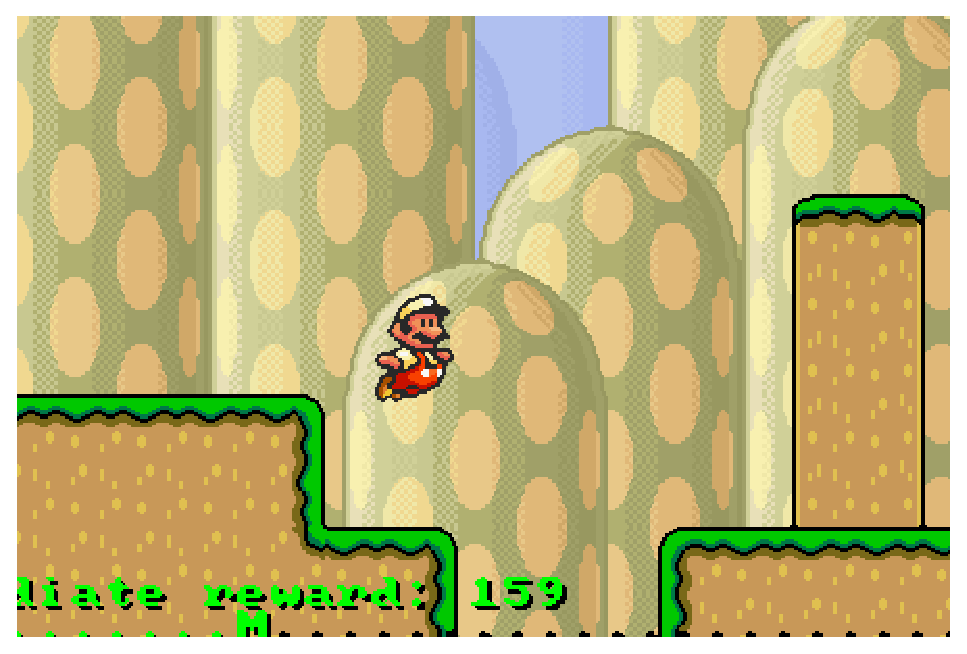
\includegraphics[scale=0.70]{figure02.eps}
\end{center}
 穴の判定は常にマリオの1マス右下であるため、普通の飛び降りの先に穴があるのを今のプログラムでは判定できない。下に降りることに対してより細かな地形判断が必要である。
 \item[$<$2$>$ 平地にポツンとある障害物の先に穴]~\\
\begin{center}
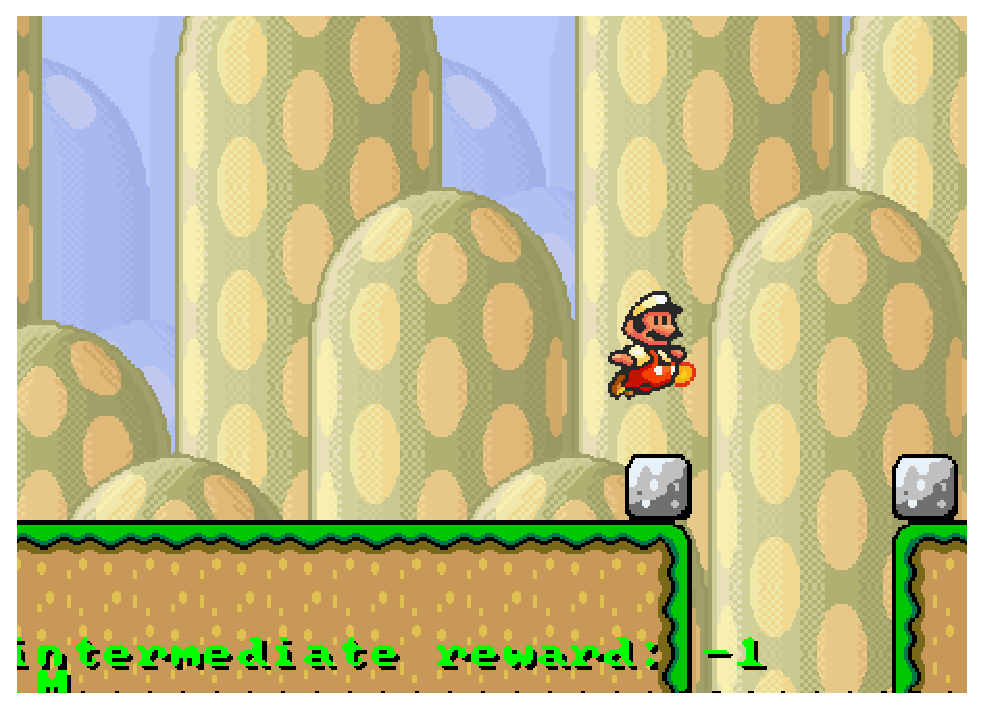
\includegraphics[scale=0.70]{figure03.eps}
\end{center}
 ジャンプの距離はジャンプボタンを押す時間だけでなく現在のマリオの速さによって決まる。平地で加速してしまったマリオは、一番小さいジャンプをであっても4,5マスは飛んでしまうため、今のプログラムでは飛びすぎが起こってしまう。ダッシュボタンを封印すれば問題はなくなるが、行動をより細かに制御することで対処したい。
\end{description}

以上の問題点などを踏まえ、全てのコースをクリアできるAIを作るために各クラスの性能を上げていくことが課題となる。
\\

感覚神経のクラスでは、より様々な地形と危険を感知できるようメソッドを増強していく必要があるだろう。マリオが到達することの出来る最も遠い足場の検出などができれば、より賢い動きができるようになることが予想される。
\\

運動神経(体)のクラスでは、ボタンの制御によってマリオがどんな状態にあっても好きな箇所に移動、着地できる自由な動きが実現できるメソッドが求められる。可能な動きが増えればより高度なクリアに繋がるため、この部分の向上は重要課題だ。
\\

脳のクラスは、向上した上記二つのクラスの制御を適切に行うようプログラム改変していく必要がある。とくに場合によって考え方を切り替えられるよう、複数の脳クラスを適宜切り替えられる仕組みの実装を予定している。
\\

以上、3つのクラスに分類した利点を最大限に活かしながら、それぞれを強化して高度なAIプログラムを実現していきたい。
%%%%%%%%%%%%%%%%%%%%%%%%%%%%%%%% 以下参考

\section{セクション}
内容

段落改行は一行あける
\subsection{サブセクション}
\subsection{サブセクション}

\subsection{箇条書き}
\begin{description}
\item [表題]~\\
内容はここに書く
\item[表題]\mbox{}\\
内容はここに書く
\item[表題に括弧を使う$<$括弧$>$]
\end{description}

\subsection{箇条書き(番号付き)}
\begin{enumerate}
\item 表題 ~\\
内容はここに書く 
\item 表題 \mbox{}\\
内容はここに書く 
\end{enumerate}

\subsection{図の挿入}
% 図のファイル名,拡大縮小率を調整する.
%\begin{center}
%  \includegraphics[scale=0.65]{figure01.eps}
%\end{center}

\subsection{スクリーン}
\begin{screen}
~\\
単純改行\\
$【括弧】$\\
$<括弧>$ \\
\end{screen}
\begin{verbatim}
文書挿入
\end{verbatim}

\end{document}
